\title{Fake News Identification}
\author{
        Username: gcdk35
}
\date{\today}

\documentclass[12pt]{article}
\usepackage{graphicx}
\usepackage{adjustbox}
\usepackage[paper=a4paper, margin=2cm]{geometry}
\begin{document}
\maketitle

\section{Data Cleaning and Representation}
The first step in both shallow and deep learning is to take the dataset given (as a CSV file), filter it,
and store the data in a way that can assist learning.

First, the entire file is loaded in, with each component being stored as a list (0 index being the index ID, 1 index being the corpus content, and 2 index being
the label).

From here, we go through the list, removing all punctuation from the corpus, leaving only words seperated by a single space, all converted to lower case.
Lower case conversion ensures that the same word is not counted differently (i.e. "Fox" will be seen as a different word to "fox" for example). Punctuation removal
ensures that punctuation doesn't cause words to be perceived as different words (e.g. "fox!" will be seen as a different word to "fox").

From here, each classifier undergoes their own specific routines, which shall be revealed in future sections.

\section{Shallow Learning Approach}
This approach uses a Multinomial Bayes Classifier, with different methods of extracting features. Each one shall be outlined below, along with the resulting accuracies.

\subsection{N Gram Only}
Features can be extracted using n-grams (a set of words). The default within sklearn is size N=1 (one word) but increasing this size does yield slightly better performance on its own.
The results, including precision, accuracy, recall and F1 scores can be found in Table \ref{ngramonly}

\begin{table}[]
        \centering
        \label{ngramonly}
        \begin{tabular}{| c | c | c | c | c | }
                \hline
                \textbf{Ngrams} & \textbf{Precision} & \textbf{Accuracy} & \textbf{Recall} & \textbf{F1}\\
                \hline
                1 & 0.885852229040716 & 0.88348594884749 & 0.88348594884749 & 0.883237395852024 \\
                2 & 0.894373523019958 & 0.877170824123776 & 0.877170824123776 & 0.875624072747213\\
                3 & 0.898585092457609 & 0.882222923902747 & 0.882222923902747 & 0.880823839680174\\
                4 & 0.883984637640072 & 0.873697505525734 & 0.873697505525734 & 0.872688593358964\\
                5 & 0.864856516164587 & 0.860435743605936 & 0.860435743605936 & 0.859890709235547\\
                \hline
        \end{tabular}
        \caption{Ngram only performance}
\end{table}

\begin{figure}
        \centering
        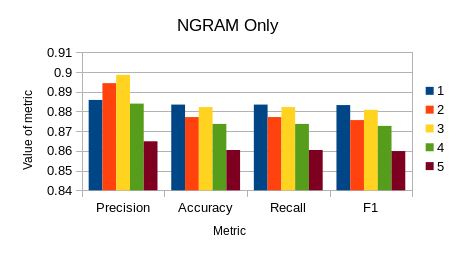
\includegraphics{ngramonly}
\end{figure}

\subsection{Term Frequency}
This automatically uses ngrams, then inputting into a Term Frequency Algorithm. Term Frequency goes through, calculating the number of times a particular
ngram has occurred in the corpus. THe intuition to this method is that more important words have a greater count that the less important ones. While this is true,
certain common words such as "the" might have a high frequency but add nothing to the overall meaning of the corpus. Therefore, stopwords are used, which are filtered from the corpus,
to ensure their presence doesn't impact the results of the output.

\begin{table}[]
        \centering
        \label{ngramonly}
        \begin{tabular}{| c | c | c | c | c | }
                \hline
                \textbf{Ngrams} & \textbf{Precision} & \textbf{Accuracy} & \textbf{Recall} & \textbf{F1}\\
                \hline
                1 & 0.855788161809308 & 0.826965582570256 & 0.826965582570256 & 0.822991482917058\\
                2 & 0.821616955256766 & 0.731922955478371 & 0.731922955478371 & 0.710538170351274\\
                3 & 0.871310793427224 & 0.838964319545311 & 0.838964319545311 & 0.835005177576252\\
                4 & 0.868394678799207 & 0.854752131354594 & 0.854752131354594 & 0.853176349640056\\
                5 & 0.856919202089254 & 0.855383643826966 & 0.855383643826966 & 0.855151105961723\\
                \hline
        \end{tabular}
        \caption{TF with NGRAMs}
\end{table}

\begin{figure}\label{tfbarchart}
        \centering
        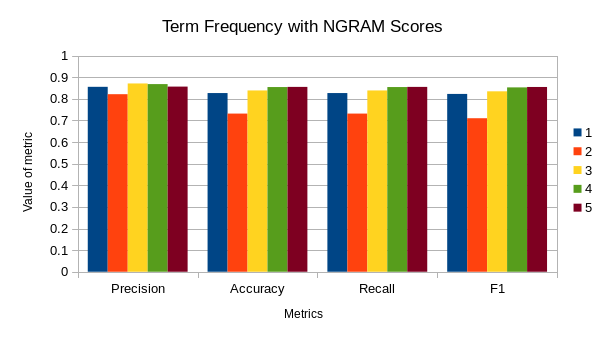
\includegraphics{tf}
        \caption{Bar chart showing metrics for Term Frequency with different ngrams}
\end{figure}


\subsection{TF-idf}
Much like Term Frequency above, this adds an additional weight to each ngram. After finding the term frequency score, we multiply it by the Inverse Document Frequency score (idf score).
The IDF score represents the amount of information a given ngram contains - if many documents contain the same ngram, then it's likely that the ngram is a common ngram, and thus not important.
This results in an advanced version of TF that automatically removes stopwords without needing to supply a list.

\textbf{TODO: table of results for TFIDF with NGRAMS}
\begin{table}[]
        \centering
        \label{ngramonly}
        \begin{tabular}{| c | c | c | c | c | }
                \hline
                \textbf{Ngrams} & \textbf{Precision} & \textbf{Accuracy} & \textbf{Recall} & \textbf{F1}\\
                \hline
                1 & 0.857713921254604 & 0.816861383012314 & 0.816861383012314 & 0.810976894429655\\
                2 & 0.849190911032834 & 0.790653615408904 & 0.790653615408904 & 0.780779400705539\\
                3 & 0.885475772379496 & 0.863909062203978 & 0.863909062203978 & 0.861732941710458\\
                4 & 0.883311761081068 & 0.875907799179034 & 0.875907799179034 & 0.875174323829035\\
                5 & 0.860056817201007 & 0.859488474897379 & 0.859488474897379 & 0.859386985721837\\
                
                \hline
        \end{tabular}
        \caption{TF with NGRAMs}
\end{table}

\begin{figure}\label{tfidfbarchart}
        \centering
        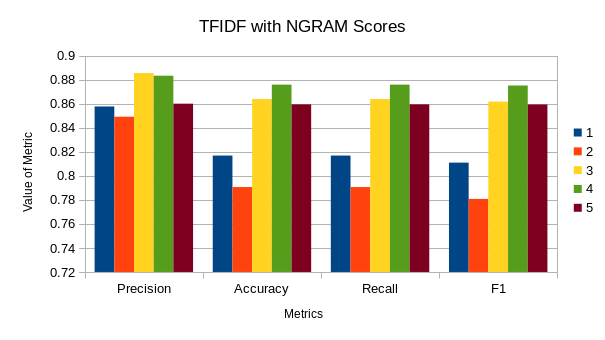
\includegraphics{tfidf}
        \caption{Bar chart showing the metrics for TFIDF for different ngrams (i.e. word amounts)}
\end{figure}

\subsection{Final Shallow Model Chosen}
Using the experiments above, looking primarily at the resulting accuracy, I chose to use only 3-grams, without using TFIDF, or TF, but using stopwords.
This not only yielded one of the highest accuracies, but the precision was also the highest. 


\section{Deep Learning}
To carry out the deep learning process, Keras was used with the Tensorflow backend.
In the case of all deep learning networks, they were trained on 60\% of the dataset, with the remaining 40\% of the data being used as test data.
This provides sufficient data to train on, but also ensures we can test the model using enough data.

Several different models were created using LSTMs.

Softmax was used for all external nodes for classification as it better represents categorical probabilities than other activations such as sigmoid.

For the extra dense layers used later on, the Hyperbolic Tangent function was used as an activation, as for largely negative input values, using a sigmoid
would yield values very near to zero, which for dense layers can cause problems (particularly without any biases). Using hyperbolic tangent instead outputs values
between -1 and 1, which better matches the domain of the values within the word2vec vectors. 

\subsection{LSTM with 100 nodes}
The outcome of using an LSTM with just 100 nodes yields an accuracy of 81\%.
\subsection{LSTM with 200 nodes}
To improve the model, increasing the number of LSTM nodes could potentially be a method of improving the 
overall model.

This yields 81\% accuracy on the test set, which doesn't really improve the performance of the system from before.
\subsection{LSTM with 200 nodes and increased dropout}
Increasing dropout might be an option, as doing this would decrease the chance of overtraining.

Increasing dropout from 0.1 to 0.2, and increasing the number of epochs from 5 to 8 yields an
accuracy of 70\%, which is considerably worse. Therefore, going back to the previous 200 node LSTM might be more ideal.

\subsection{LSTM with larger dense layer}
Instead of just passing the output of the LSTM (with 200 nodes) straight to the dense layer with 2 nodes, we put a layer with 100 nodes between these two layers,
the idea being to provide further weights and nodes to train a more complex model. Results by adding this layer increased, yielding an 83\% accuracy on the test data.

This is the final solution for my LSTM code, which in my experimentation performed the best.

\subsection{RNN vs LSTM}
Above, an LSTM was used, which yielded the best results.

Replacing the LSTM layer with an RNN layer (SimpleRNN in Keras), not including the 100 node dense layer,
yielded a performance that wasn't as good as the LSTM, but the training time was far quicker. The accuracy score for an RNN was
70.3\%, definitely worse than any of the previous LSTM scores. This is to be expected, as LSTMs are essentially RNNs that also have
memory that lasts over a longer period, perhaps meaning that the classification with the RNN was more local (as earlier words no longer fully 
existed in terms of memory inside of the network). 

More specifically, performance wise this model took 947 seconds, far better than the 2792 seconds for the LSTM.
\section{Performance of Shallow vs Deep}
Overall, I found that the Shallow Learning approach was far better for this problem. Using this method, training was considerably quicker, taking only 14 seconds when compared with the 2792 seconds for the deep learning solution.
The outcome was also far better when compared with deep learning (88\% accuracy with ngram only multinomial training when compared with 83\% for the deep learning solution proposed).
When using an RNN, the performance was better, but yielded far worse results, and shallow outperformed both deep learning models on both performance and accuracy.

Hence, for this system, I'd say that the more Naive Multinomial Bayes approach is far better, as the performance is better, but also yields far better results.

\end{document}